\chapter{Critical Success Factor Analysis Based on Feaure Selection}
\label{ch:2_csf_fs}

\begin{quotation}[]{Paulo Freire}
No one knows it all. No one is ignorant of everything. We all know something. We are all ignorant of something.
\end{quotation}

Critical Success Factor (CSF) is a management term for an element that is necessary for an organization or project to achieve its mission. CSFs represent the principal assets or areas that must be given investments to achieve better results. CSF analysis is one challenger strategic management tool, wich can provide a robust and very practical assessment for strategic planners.

The identification of the most significative information for one problem is referred to as feature selection by the signal processing and data mining areas, as well as it can be formulated as a principal component problem, which is a widely adopted signal processing technique for data visualization and feature extraction. Feature selection aims to select a subset of relevant information from a larger dataset, in order to improve: data visualization and data understanding, storage requirements, dimensionality, processing time, discriminative sensing, and to overcome overfitting problems to improve prediction and classification performance \cite{chandrashekar2014survey}.

Recursive Feature Elimination (RFE) is a feature selection method for small sample classification problems. RFE seeks to improve generalization performance by recursivelly removing the least significant features whose deletion will have the least effect on training errors, according to the higher variance measured from the features \cite{chen2007enhanced}.

We propose a critical factors analysis based on Principal Compoment Analytis (PCA) for visual discriminant analysis and based on RFE combined with Support Vector Machine (SVM) \cite{hearst1998support}, applied to the survey that evaluates the IT governance of brazilian public organizations, in order to identify the CSF for IT governance of the public sector according to TCU. Results show how PCA can make the data discriminative and that SVM is the classifier that best performs and obtains an accuracy of 91.42\% to learn and classify according to TCU's IT governance evaluation of brazilian public sector. Finally, SVM is used to highlight the more significant features identified by RFE, wich are limilar to CSFs previsously identified by a qualitative analysis of the same datased.

This chapter is organized as follows. In Section \ref{sec:ch2_relatedworks}, related works are discussed. Section \ref{sec:ch2_datamodel} presents the data model and the evaluated datasets. Section \ref{sec:ch2_csf_fs} describes the proposed approach for critical success factors analysis. Section \ref{sec:ch2_experimentalresults} discusses the experimental validation and presents the results, and Section \ref{sec:ch2_conclusion} draws the conclusions.

\section{Related Works}
\label{sec:ch2_relatedworks}

Fink and Sukenik \cite{fink2011effect} explore the relationships among IT infrastructure capability and IT business value using PCA applied to all indicators of their study, resulting into 11 factors, with the first factor accounting for only 27.9\% of the variance. This technique was used because the PCA extracts orthogonal factors that overcome the problem of multicollinearity.

Ramos \emph{et al} \cite{ramos2016information} propose an overview regarding the evolution of scientific research on IT Governance critical success factors within the domain of public administration. By means of bibliometric analysis it was investigated seminal works regarding this theme, considering the characteristic key words found during our analysis. The results present 64 critical success factors with high impact on IT governance.

Guyon \emph{et al} \cite{guyon2002gene} propose a method of gene selection utilizing Support Vector Machine methods based on Recursive Feature Elimination (RFE) and demonstrate that the selected genes yield better classification performance and are biologically relevant to cancer.  The proposed method eliminates gene redundancy automatically and yields better and more compact gene subsets. 

To the best of our knowledge, we are the first to propose a critical factors analysis based on PCA for visual discriminant analysis and based on RFE combined with SVM for CSF identification from IT governance data.

\section{Data Model}
\label{sec:ch2_datamodel}

The brazilian Federal Court of Accounts (TCU, in Portuguese) surveys data regarding IT practices of brazilian public organizations in order to audit IT governance. The dataset with a consolidate view about the answers for this surgey the IT governance index is called iGovTI. The iGovTI is composed by 201 multiple choice questions, used for ranking according to their IT governance, submmited to 349 organizations. The TCU computes the IT governance index and classifies the IT governace of each organization. Additionally, Ramos \emph{et al} \cite{ramos2016information} classifies each question regarding its relevance for IT governance through a qualitative analysis, and identify the CSFs for selected IT managers regarding IT governance.

\section{An approach for Critical Success Factors Analysis}
\label{sec:ch2_csf_fs}

In this section we propose an approach for CSF Analysis based on visual discriminant analysis and based on feature selection, in order to identify the CSFs for IT governance according to iGovTI. Initially we conduct an analysis based on PCA to evaluate the relevance of each question according to their variance, and use the 2 most relevant features for a visualization of the iGovTI ranking. Furthermore, we propose a critical success factors analysis based on SVM for classification and based on RFE for identification of the most relevant factors.

\subsection{Visual Discriminant Analysis based on PCA}
\label{sec:ch2_pca}

PCA is a statistical technique commonly used for signal denoising, blind source separation, data compression, data visualization, feature extraction and dimensionality reduction, where a reduced number of features is extrated retaining as much information as possible \cite{jolliffe1986principal}. It uses an orthogonal transformation to convert a set of correlated variables into a set of linearly uncorrelated variables, where the first principal components have the largest variance.

PCA is an orthogonal basis transformation into new basis, by diagonalizing the centered covariance matrix of a data set \{$\mathbf{x}_j \in \mathbb{R}^m, j = 1, ... ,n$\}, defined by $\mathbf{C} = \frac{\mathbf{X}^\intercal\mathbf{X}}{n}$, where $\mathbf{X} = (\mathbf{x}_1, ... , \mathbf{x}_n)^\intercal$ and the samples are assumed to have zero mean. The eigenvectors $\mathbf{v}_i$ of $\mathbf{C}$ are called principal components (PC), and the sample variance along $\mathbf{v}_i$ of $\mathbf{C}$ is given by the corresponding eigenvalue $\lambda_i$. Projecting onto the eigenvectors with the largest eigenvalues assumes that minimal information is lost, considering that in many applications these directions contain the most interesting information, such as in in data compression and de-noising.

Initially, we compute the covariance matrix $\mathbf{C}$ of a zero mean data and visualize the data relationship for the sambple covariance. Sample covariance is calculated by computing deviations of each measurement from the average of all measurements for that variable. Then the deviations for the two measurements are multiplied together separately for each subject. Finally these values are averaged. After that, the eigenvectors $\mathbf{v}_i$ and eigenvalues $\lambda_i$ of $\mathbf{C}$ are computed through Singular Value Decomposition (SVD), then it is possible to evaluate the variance distribution of the extracted components through an empirical cumulative distribution function (ECDF). Evaluating the variance distribution we expect to visualize if some features concentrates the variance and indicates advantages for dimensionality reduction.

Finally, we propose to select the two features with the largest variance and evaluate the relationship between the two principal components and the iGovTI classification, in order to visualize if there is a segmentation according to the iGovTI ranking.

Considering that PCA combines attributes and creates new ones, with measurements from all of the original variables, it is hard to identify what original variables are most relevant. Therefore, it is still necessary an additional method to reveal what are the CSF for iGovTI. For this problem, we propose a CSF analysis based on RFE.

\subsection{CSF analysis based on RFE}
\label{sec:ch2_csfa}

Feature selection aims the identification of the most significative information for one problem or algorithm, such as classification or prediction problems. RFE is a feature selection method for small sample classification problems by recursivelly removing the least significant features whose deletion will have the least effect on training errors, according to the higher variance measured from the features through a selected classifier. 

Initially, it is necessary to identify one classifier that can identify the iGovTI classificatin of one organization according to a trainning dataset. Therefore, we propose an algorithm evaluatio in order to identify wich one presents the best accuracy for iGovTI classification. The selected algorithm should be used by RFE to identify the CSF, that should be compared to results of the CSF qualitative analysis conducted by Ramos \emph{et al} \cite{ramos2016information}.

Feature selection doesn't combine attributes, as PCA, but just evaluates their informative quality, predictive power and select the best set. Given an external estimator or classifier, that assigns weights to features, RFE is able to select features by recursively considering smaller and smaller sets of features. First, the estimator is trained on the initial set of features and the importance of each feature is obtained either through a coefficient attribute or through a feature importances attribute. Then, the least important features are pruned from current set of features. That procedure is recursively repeated on the pruned set until the desired number of features to select is eventually reached. RFE can also rank all features areaccording to when they were eliminated. 

The variables with the least effect on training errors or largest weights indicates more relevance for a classifier. Therefore, we propose to assume that the selected most relevant features are the CSF for iGovTI and also propose to validate this assumption against the results of the CSF qualitative analysis conducted by Ramos \emph{et al} \cite{ramos2016information}.

\section{Experiments and Results}
\label{sec:ch2_experimentalresults}

In this section we present the experiements and results for the visual discriminant analysis based on PCA and for CSF analysis based on RFE, and discuss the results.

For the visual discriminant analysis we initially we compute the zero mean and then compute the correlation matrix $\mathbf{C}$ is computed from $\mathbf{X}$, which is shown by Figure \ref{fig:ch2_fig1}.
 
\begin{figure}[h!]
     \centering 
     \includegraphics[height=10cm, width=10cm]{figures/ch2/raw_igovti_covariance.eps}
     \caption{Covariance matrix of iGovTI questions.}
     \label{fig:ch2_fig1}
\end{figure}

Figure \ref{fig:ch2_fig1} presents the matrix presents of 201 questions of iGovTI, where is possible to observe low covariance for the majority questions and high variance for just a few variables. The low covariance reveals

Depois da extração dos autovalores e percentual da variância explicada, é decidida a quantidade de fatores a serem retirados para análise. Para isso, o Gráfico 1 em que o total de autovalores está no eixo das ordenadas e os autovalores  no eixo das abscissas, auxilia na identificação. Esse gráfico consiste no ranking dos autovalores (eixo x), relacionado com o valor de cada autovalor (eixo y). Verifica-se que uma queda menos acentuada ocorreu entre o quarto e o quinto autovalor e analisando-se os autovalores superiores a 2, observa-se que pode-se considerar até o vigésimo valor já que a partir daí os valores dos autovalores sucessivos são praticamente constantes.

\begin{figure}[h!]
     \centering 
     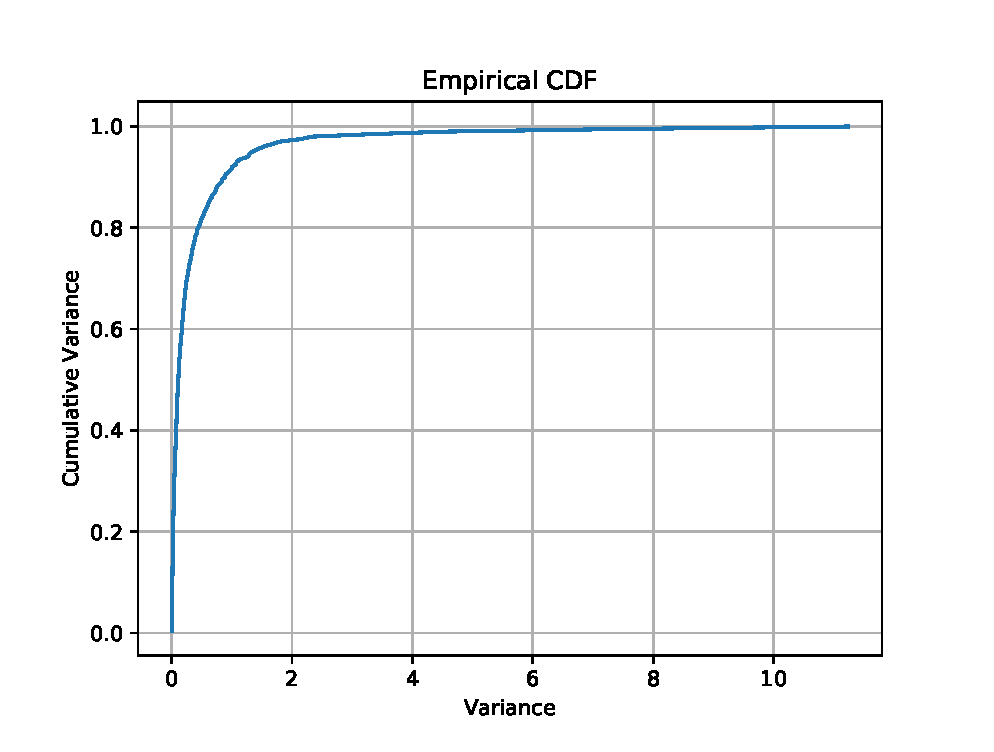
\includegraphics[height=8cm, width=11cm]{figures/ch2/raw_variance_ecdf.eps}
     \caption{Empirical CDF of variance.}
     \label{fig:ch2_fig2}
\end{figure}
 
Visando encontrar os planos fatoriais realizou-se uma rotação dos eixos, onde as cargas fatoriais mais elevadas são as responsáveis pelas denominações das componentes e são estatisticamente significativas. As rotações de eixos melhor expressam a dispersão de dados. No modelo fatorial final, as variáveis das medidas estão maximizadas e as relações entre dimensões suavizadas (Vicini, 2005).
Para esta análise buscam-se valores que possuem significância maior que 0,7, mostrando que a correlação entre as variáveis está de moderada a forte (Vicini, 2005). Essa identificação não seria possível sem a rotação dos eixos, possibilitando assim a melhor visualização das variáveis mais significativas em cada componente. Tal rotação mantem os eixos perpendiculares entre si, ou seja, ortogonais e a variabilidade do sistema não é alterada, apenas as coordenadas dos eixos são rotacionadas e a inércia do sistema fica inalterada. 
A partir dos valores obtidos pela rotação das componentes principais, podem-se obter valores com significância maior que 0,7. Logo, foi possível a identificação das variáveis significantes de cada componente principal.
Para visualização desses fatores foi utilizado o gráfico de dispersão (Gráfico 2). O Gráfico 2 mostra a caixa de seleção de variáveis e comandos para ACP em que se utilizam os fatores 1 e 2, eixo x e eixo y respectivamente. O objetivo deste gráfico é fazer os planos principais com a nuvem de pontos dos indivíduos, no caso as 349 instituições, destacando o posicionamento das respostas das instituições classificadas pelo iGovTI. Tal gráfico se baseia na rotação dos componentes principais. Para a elaboração do Gráfico 2 apenas os  e  foram utilizados.
 
\begin{figure}[h!]
     \centering 
     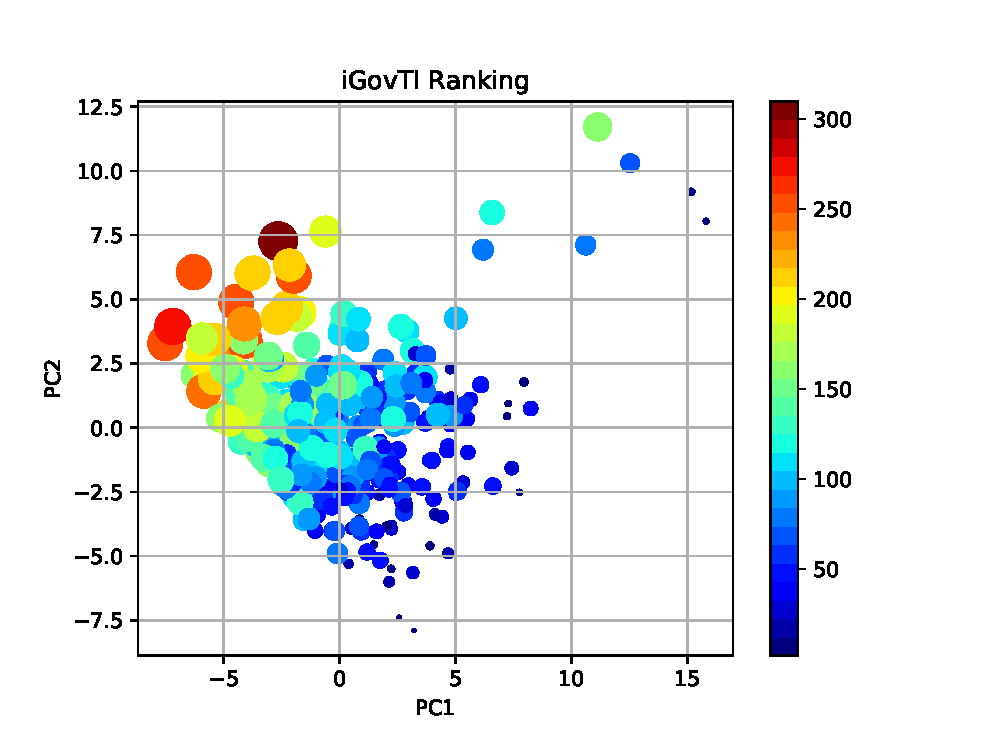
\includegraphics[height=8cm, width=11cm]{figures/ch2/raw_igovti_ranking_pc2.eps}
     \caption{iGovTI ranking from 2 principal components.}
     \label{fig:ch2_fig3}
\end{figure}

No Gráfico 2, para analisar apenas a , projetam-se os pontos sobre o eixo da e se tem três grupos (V, II e I). O mesmo processo se aplica a analise da . Assim, observam-se três grupos (V, IV e III). Para cada grupo se seleciona apenas uma variável representativa, o restante é desconsiderado, uma vez que cada grupo significa correlação.
Para o grupo I, tomam-se as variáveis Q16d, Q16e e Q16f que são descorrelacionadas, já no grupo II a questão Q16g é questão selecionada. Ambos os grupos não apresentam FCS. Essas questões denotadas Q16, referem-se a Subdimensão 1.6 (A Alta Administração Utilizou Informações Fornecidas pela Auditoria Interna). Tal subdimensão verifica a participação da auditoria interna das instituições para o preenchimento do questionário. 
% Já no grupo III, que não tem FCS, a variável Q53_Relev é a selecionada; precedidas do grupo IV que também não apresenta FCS. Ressalta-se que ambas as questões apuram a relevância de determinado item. Pela análise ACP, o grupo V mostra as questões que não são representadas pelas  e , é justamente este grupo que contem os FCS.
Depois, buscou-se por meio da análise das ,  e a identificação de FCS (Gráfico 3). O Gráfico 3 mostra a análise dessas componentes principais que revela a existência de três grupos. 

A análise do Gráfico 3 mostra revela a existência de três grupos (VI, VII e VIII). O grupo I contém a variável Q51l que corresponde a FCS e o grupo II também mostra FCS, a variável Q23b.
Na identificação das variáveis significativas das primeiras 20 componentes principais, com os autovalores superiores a 1, as questões que mais contribuem são Q16b (para responder às questões do grupo 2. Estratégias e planos), Q16c (para responder às questões do grupo 3. Informação e conhecimento), Q16d (para responder às questões do grupo 4. Pessoas), Q16e (para responder às questões do grupo 5. Processos) e Q16f (para responder às questões do grupo 6. Resultados da gestão), todas da dimensão “Governança corporativa e de TI, a alta administração utilizou informações fornecidas pela auditoria interna (ou instância equivalente)”. Nota-se que as variáveis Q16, citadas anteriormente, fazem parte do grupo I do Gráfico 2. Ao total foram identificadas 29 variáveis dos 20 primeiras componentes principais (autovalores maiores que 1) das variáveis com significância maior que 0,7. O Quadro 8 mostra quais são essas variáveis significativas. 

No Quadro 8, verificou-se as variáveis que são FCS, de acordo com resultado da pesquisa apresentada na Subseção 4.1. Das 30 questões apenas 5 são FCS, de acordo com classificação obtida por meio de pesquisa qualitativa, quais sejam: Q12c (designou representantes de todas as áreas relevantes para o negócio institucional para compor o Comitê de TI); Q23b (a instituição aprovou e  publicou PDTI interna e externamente); Q51l (gestão de configuração de ativos); Q53e (formalizou a política corporativa de segurança da informação); Q57h (os pagamentos são feitos em função da mensuração objetiva dos resultados entregues e aceitos.
Ainda no Quadro 8, chama-se atenção as ,  e. Nelas constam variáveis com valor positivo ou negativo. Tal fato significa que quanto maior for a resposta de uma questão menor será a da outra. Frisa-se que isto só vale para questões que estejam em uma mesma variável ACP. Caso as questões tenham sinais diferentes (i.e. os elementos dos autovetores), mas em ACP diferentes o sinal positivo e negativo não importa. 
A análise das categorias (Quadro 5) relacionadas às variáveis revela: Q53e referente à Categoria Processos de Gestão de Serviços de TI em Desenho do Serviço que mostrou porcentual igual a 53,85\%; Q57h se liga à Categoria Gestão de Contratos que teve porcentual de 38,46\%; Q23b se vincula à Categoria PDTI que teve 38,46\%. A variável Q51l se relaciona à Categoria Processos de Gestão de Serviços de TI em Transição de Serviços com 19,23\%.
Devido ao baixo percentual de 16,66\% de identificação de FCS do Quadro 8, realizou-se a análise das variáveis que completam as 51 componentes principais, referentes aos 51 autovalores do Quadro 7. Nesta identificação, foram identificadas 33 variáveis, sendo que 8 são FCS, 24,24\% (Quadro 9). Somando os totais obtidos pelo Quadro 8 e pelo se tem, 20,63\% de variáveis que são FCS.

Já o Gráfico 4 mostra a caixa de seleção de variáveis e comandos para ACP em que se utilizam os fatores 1 e 2, eixo x e eixo y respectivamente. O objetivo deste gráfico é fazer os planos principais com a nuvem de pontos dos indivíduos, no caso as 349 instituições.  

O Gráfico 4 representa a relação entre os 2 principais componentes, que representam as questões ou variáveis com maiores autovalores, assim cada ponto representa a relação entre uma instituição e seus 2 principais componentes obtidos por meio de ACP. Cada ponto deste gráfico representa a classificação da instituição em relação a sua classificação no iGovTI de 2012. A partir do resultado apresentado no gráfico 4 é possível identificar um padrão formado pela localização dos componentes principais das organizações com maior índice, onde as organizações com maior iGovTI tiveram valores relativamente semelhantes para seus 2 componentes principais, entretanto ainda não é possível obter uma separação clara entre os resultados. Fazendo-se um corte no eixo das abcissas, a partir do ponto (-8,8, 0), destacam-se 23 instituições à esquerda desse ponto (Quadro 5). 

Dessas instituições, 22, são consideradas pelo TCU como aprimoradas, ou seja, 95,65\%. Apenas a instituição 346 é avaliada como intermediária.
Após a análise ACP, verifica-se que a mesma não é útil para a análise da Hipótese 2. Para responder a essa hipótese, é necessária a execução dos algoritmos de classificação da Subseção 4.4 e da Subseção 4.5.

Para prever a classificação de uma instituição de acordo com suas respostas para as questões do questionário iGovTI, foram avaliados algoritmos de classificação que pudessem apresentar acurácia para a classificação de organizações de acordo com o iGovTI. Uma vez encontrado um algoritmo capaz desta classificação, é possível utilizar o algoritmo selecionado em conjunto com técnicas de feature selection para identificar as questões mais relevantes para a classificação da instituição de acordo com o iGovTI.
Assim, para a definição do algoritmo de classificação foram realizados testes em 21 algoritmos, a seguir é apresentada uma listagem dos algoritmos avaliados e a taxa de acerto de classificação obtida: 

\begin{table*}[!t]
	\caption{Evaluation of classification accuracy for iGovTI}
  	\label{tab:ch2_tab3}
	\centering
	\begin{tabular}{|l|r|}
		\hline \rowcolor{Gray} Algorithm	& Mean Accuracy\\\hline
		Linear Regression \cite{draper2014applied}	&0.3608\\ \hline
		LDA \cite{martinez2001pca}	&0.6285\\ \hline
		K-Nearest Neighbors \cite{fukunaga1975branch}	&0.7142\\ \hline
		Linear SVM \cite{fan2008liblinear}	&0.7142\\ \hline
		Logistic Regression \cite{hosmer2013applied}	&0.7714\\ \hline
		SVM Regression \cite{smola2004tutorial}	&0.8268\\ \hline
		Lasso \cite{tibshirani1996regression}	&0.8274\\ \hline
		Elastic Net \cite{zou2005regularization}	&0.8315\\ \hline
		SVM \cite{hearst1998support}	&0.9142\\ \hline
	\end{tabular}
\end{table*}

MVS-ERV (Guyon, 2002) é uma aplicação da ERV utilizando os pesos obtidos por meio do treinamento utilizando MVS como algoritmo de classificação, para identificar as variáveis mais importantes para predições de classificação e eliminar recursivamente as variáveis que menos influenciam na classificação.. Falar que SVM-RFE é um algoritmo bem estabelecido e que concidentemente foi o melhor avaliado para este caso. SVM já é proposto para small datasets, o que foi validado com o nosso caso.

O algoritmo que obteve maior sucesso para classificação foi o SVC, que é uma implementação de Máquina de Vetores de Suporte aplicado para a classificação. SVC apresentou uma taxa de acerto de 91,4\%. Para a avaliação dos algoritmos, utilizamos uma metodologia que divide os dados dos questionários pelo iGovTI entre questões que serão utilizadas para aprendizado do algoritmo e questões que serão utilizadas para comparativo de predições. Para treinar o algoritmo utilizou-se 90\% dos dados e os 10\% restantes foram utilizados para avaliar a eficiência de classificação dos algoritmos, comparando a taxa de acerto entre as predições feitas e os valores reais de classificações de organizações pelo iGovTI. 

Uma vez identificado um algoritmo capaz de efetuar a classificação desejada, o próximo passo é identificar as variáveis mais relevantes para esta classificação. Para isso, será utilizado o algoritmo ERV. 

A ERV pode usar vários algoritmos de classificação como critério de seleção das variáveis mais importantes, escolhemos o algoritmo SVC por ele ter apresentado maior acurácia entre os algoritmos de classificação avaliados. Ainda é necessário definir o quantitativo de variáveis mais importantes a serem selecionadas. A partir da pesquisa de identificação por meio de entrevistas na APF, identificou-se 54 variáveis consideradas FCS, este critério foi utilizado para determinar o quantitativo de variáveis mais importantes para a classificação.

Assim, aplicaram-se o algoritmo ERV utilizando o SVC como critério para a seleção das variáveis mais importantes para a classificação, selecionando as 54 variáveis que correspondem aos FCS levantados nas entrevistas com os executivos de TI. Os resultados mostraram que 69,9\% das variáveis foram classificadas da mesma forma que os FCS identificados anteriormente (Quadro 10) por meio de pesquisa qualitativa.

\section{Conclusion}
\label{sec:ch2_conclusion}

pca make possible visual discriminative analysis of reduced dataset but it is not easy make correlation betwee extracted features and its original, therefore it is necessary adictional techniques to identify CSF.

SVM have been shown to generalize well even for small sample classification[8]. SVM presents high performance to reproduce the iGovTI classification and can be used for RFE in order to identify CSF

The selected features revealed by RFE are quite similar to the qualitative analysis of Ramos \emph{et al} \cite{ramos2016information}.

Question with low variance can indicate that it is irrelevant for evaluation, since its value is almost the same all the time